\newpage
\section{Realisering}
\label{realiseringOgTest}

\subsection{Kretsopkobling}
Oppkoblingen ble gjort som vist i den prinsippielle løsningen i \autoref{fig:diffamp}, hvor strømkliden ble realisert som i \autoref{fig:CurrentSource}. Hvor $Q_5$ og $R_{I1}$ fungerer som en strømkilde som er styrt av spenningen som er mellom $R_{I2}$ og $R_{I3}$, hvor $R_{I2}$ ble realisert som et potensiometer for å lettere kunne justere strømstyrken underveis. Modellnummer og komponent verdiene som ble brukt i oppkoblingen vises i \autoref{tab:komnpomenter}.  

\begin{figure}[H]
    \centering
    \begin{minipage}[c]{0.4\textwidth}
        \centering
        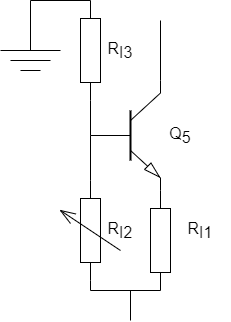
\includegraphics[width=0.6\textwidth]{Bilder/current_source.drawio.png} 
        \caption{Realisert strømkilde.}
        \label{fig:CurrentSource}
    \end{minipage}
    \begin{minipage}[c]{0.4\textwidth}
        \begin{table}[H]
            \caption{Komponenter og verdier brukt i designet.}
            \label{tab:komnpomenter}
            \begin{tabular}{ |c|c| }
                \hline
                Komponent & Verdi/Produknummer \\ \hline
                \hline
                $Q_1 \& Q_2 \&Q_5$ & BC547A (NPN) \\
                $Q_3 \& Q_4$ & BC557B (PNP) \\
                $R_{I1}$ & $3\text{k}\Omega $ \\
                $R_{I2}$ & $0\Omega - 10\text{k}\Omega$ \\
                $R_{I3}$ & $10\text{k}\Omega$ \\
                \hline
            \end{tabular}
            
        \end{table}
    \end{minipage}
\end{figure}

Den oppkoblede kretsen vises i \autoref{fig:diffamp_realisert}.

\begin{figure}[!h]
    \centering
    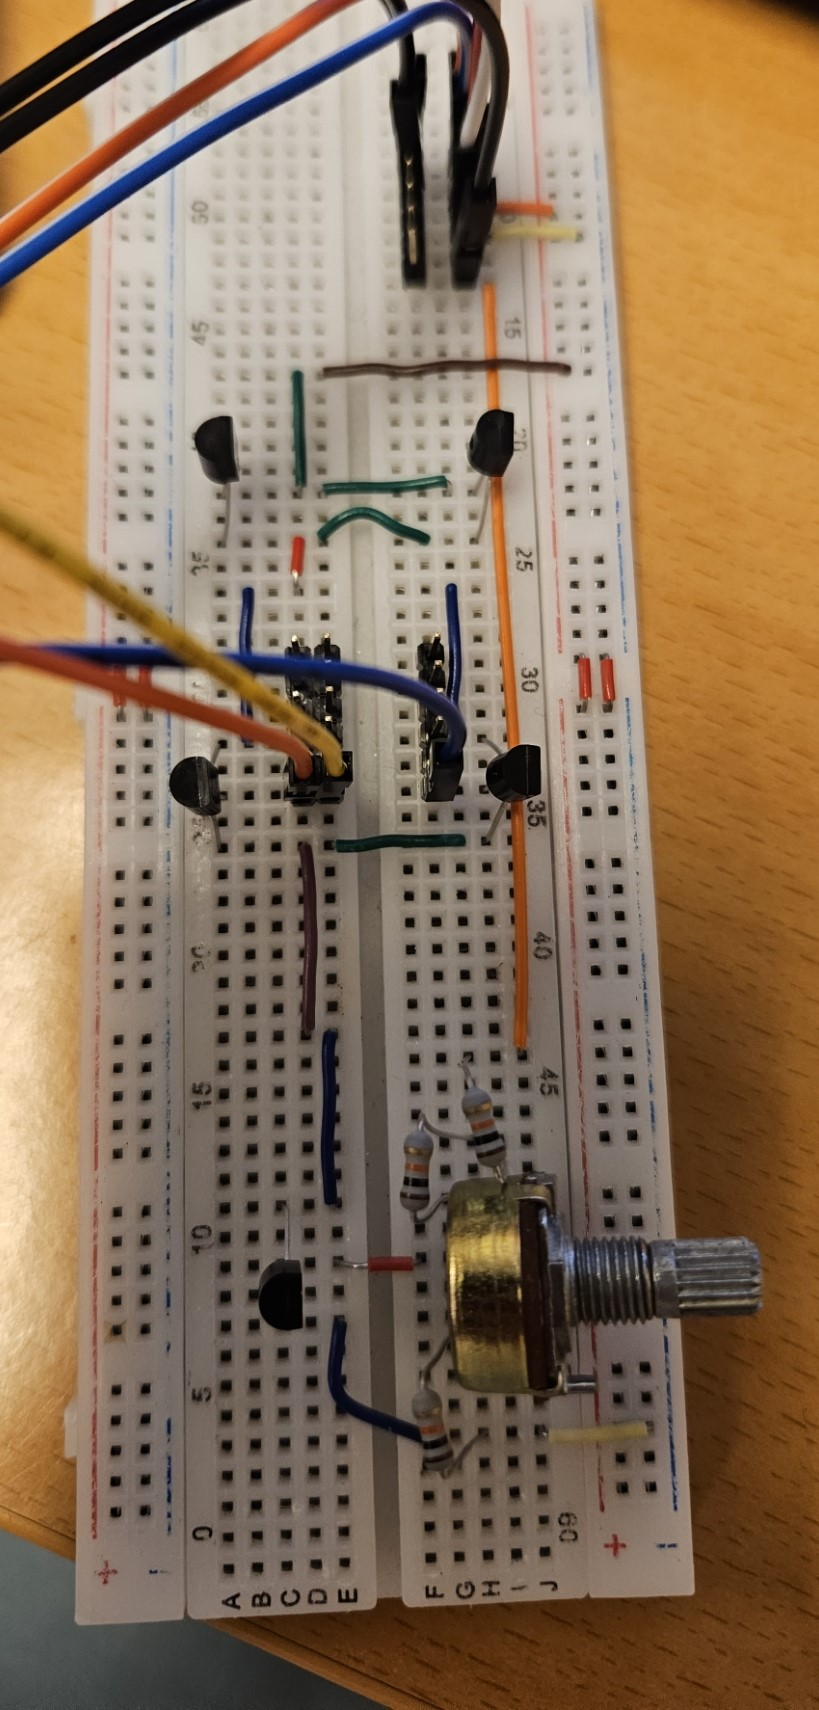
\includegraphics[width=0.4\textwidth, angle=90]{Bilder/feilBilde.jpg}
    \caption{Realisert opperasjonsforsterker}
    \label{fig:diffamp_realisert}
\end{figure}

\clearpage
\subsection{Målinger}
Det ble gjort målinger med ocilioskop og spektrumsanalysator, derretter ble målingene prosesert i python for å finne THD og forsterkning. Målingene ble gjort med en inngangsamplitude på 0.04V og en frekvens på 1kHz. Resultatene av målingene vises i tabell \autoref{tab:THD_and_Amplitude_Data}. Ut av tabellen kan vi se at forsterkningen varierer mye når vi ikke har tilbakekobling på utgangen og når vi setter på en lav lastmotstand så synker forsterkningen kraftig. Spektrumsanalysen av utgagnssignalet med last på $R_L = 100k\Omega$ både med og uten tilbakekobling vises i figur \autoref{fig:Spectrum_OPAMP_1_tilbake_100KOhm} og i figur \autoref{fig:Spectrum_OPAMP_1_100KOhm}. 
%Vi ser at THD er mye lavere med tilbakekobling enn uten. Dette er fordi tilbakekoblingen reduserer forsterkningen, og dermed reduseres også forsterkningen av harmoniske signaler.

\begin{table}[h!]
    \centering
    \begin{tabular}{ |c|c|c|c|c| }
        \hline
        Konfigurasjon & Amplitude inn & Amplitude ut & Forsterkning &THD\\
        \hline
        $R_L = 0$ & 0.04V & 0.90V & 20 &1.38\% \\
        $R_L = 100k\Omega$ & 0.04V & 0.99V & 22& 0.78\% \\
        $R_L = 100\Omega$ & 0.04V & 0.72V & 16& 10.67\% \\
        \hline
        Tilbakekobling $R_L =0$& 0.04V & 0.42V & 9.7& 1.33\% \\
        Tilbakekobling $R_L =100k\Omega$ & 0.04V & 0.42V & 9.4& 0.41\% \\
        Tilbakekobling $R_L =100\Omega$ & 0.04V & 0.21V & 4.7& 0.54\% \\
        \hline
    \end{tabular}
    \caption{THD and Amplitude Data}
    \label{tab:THD_and_Amplitude_Data}
  \end{table}

\begin{figure}[!h]
    \begin{minipage}[c]{0.5\textwidth}
        \centering
        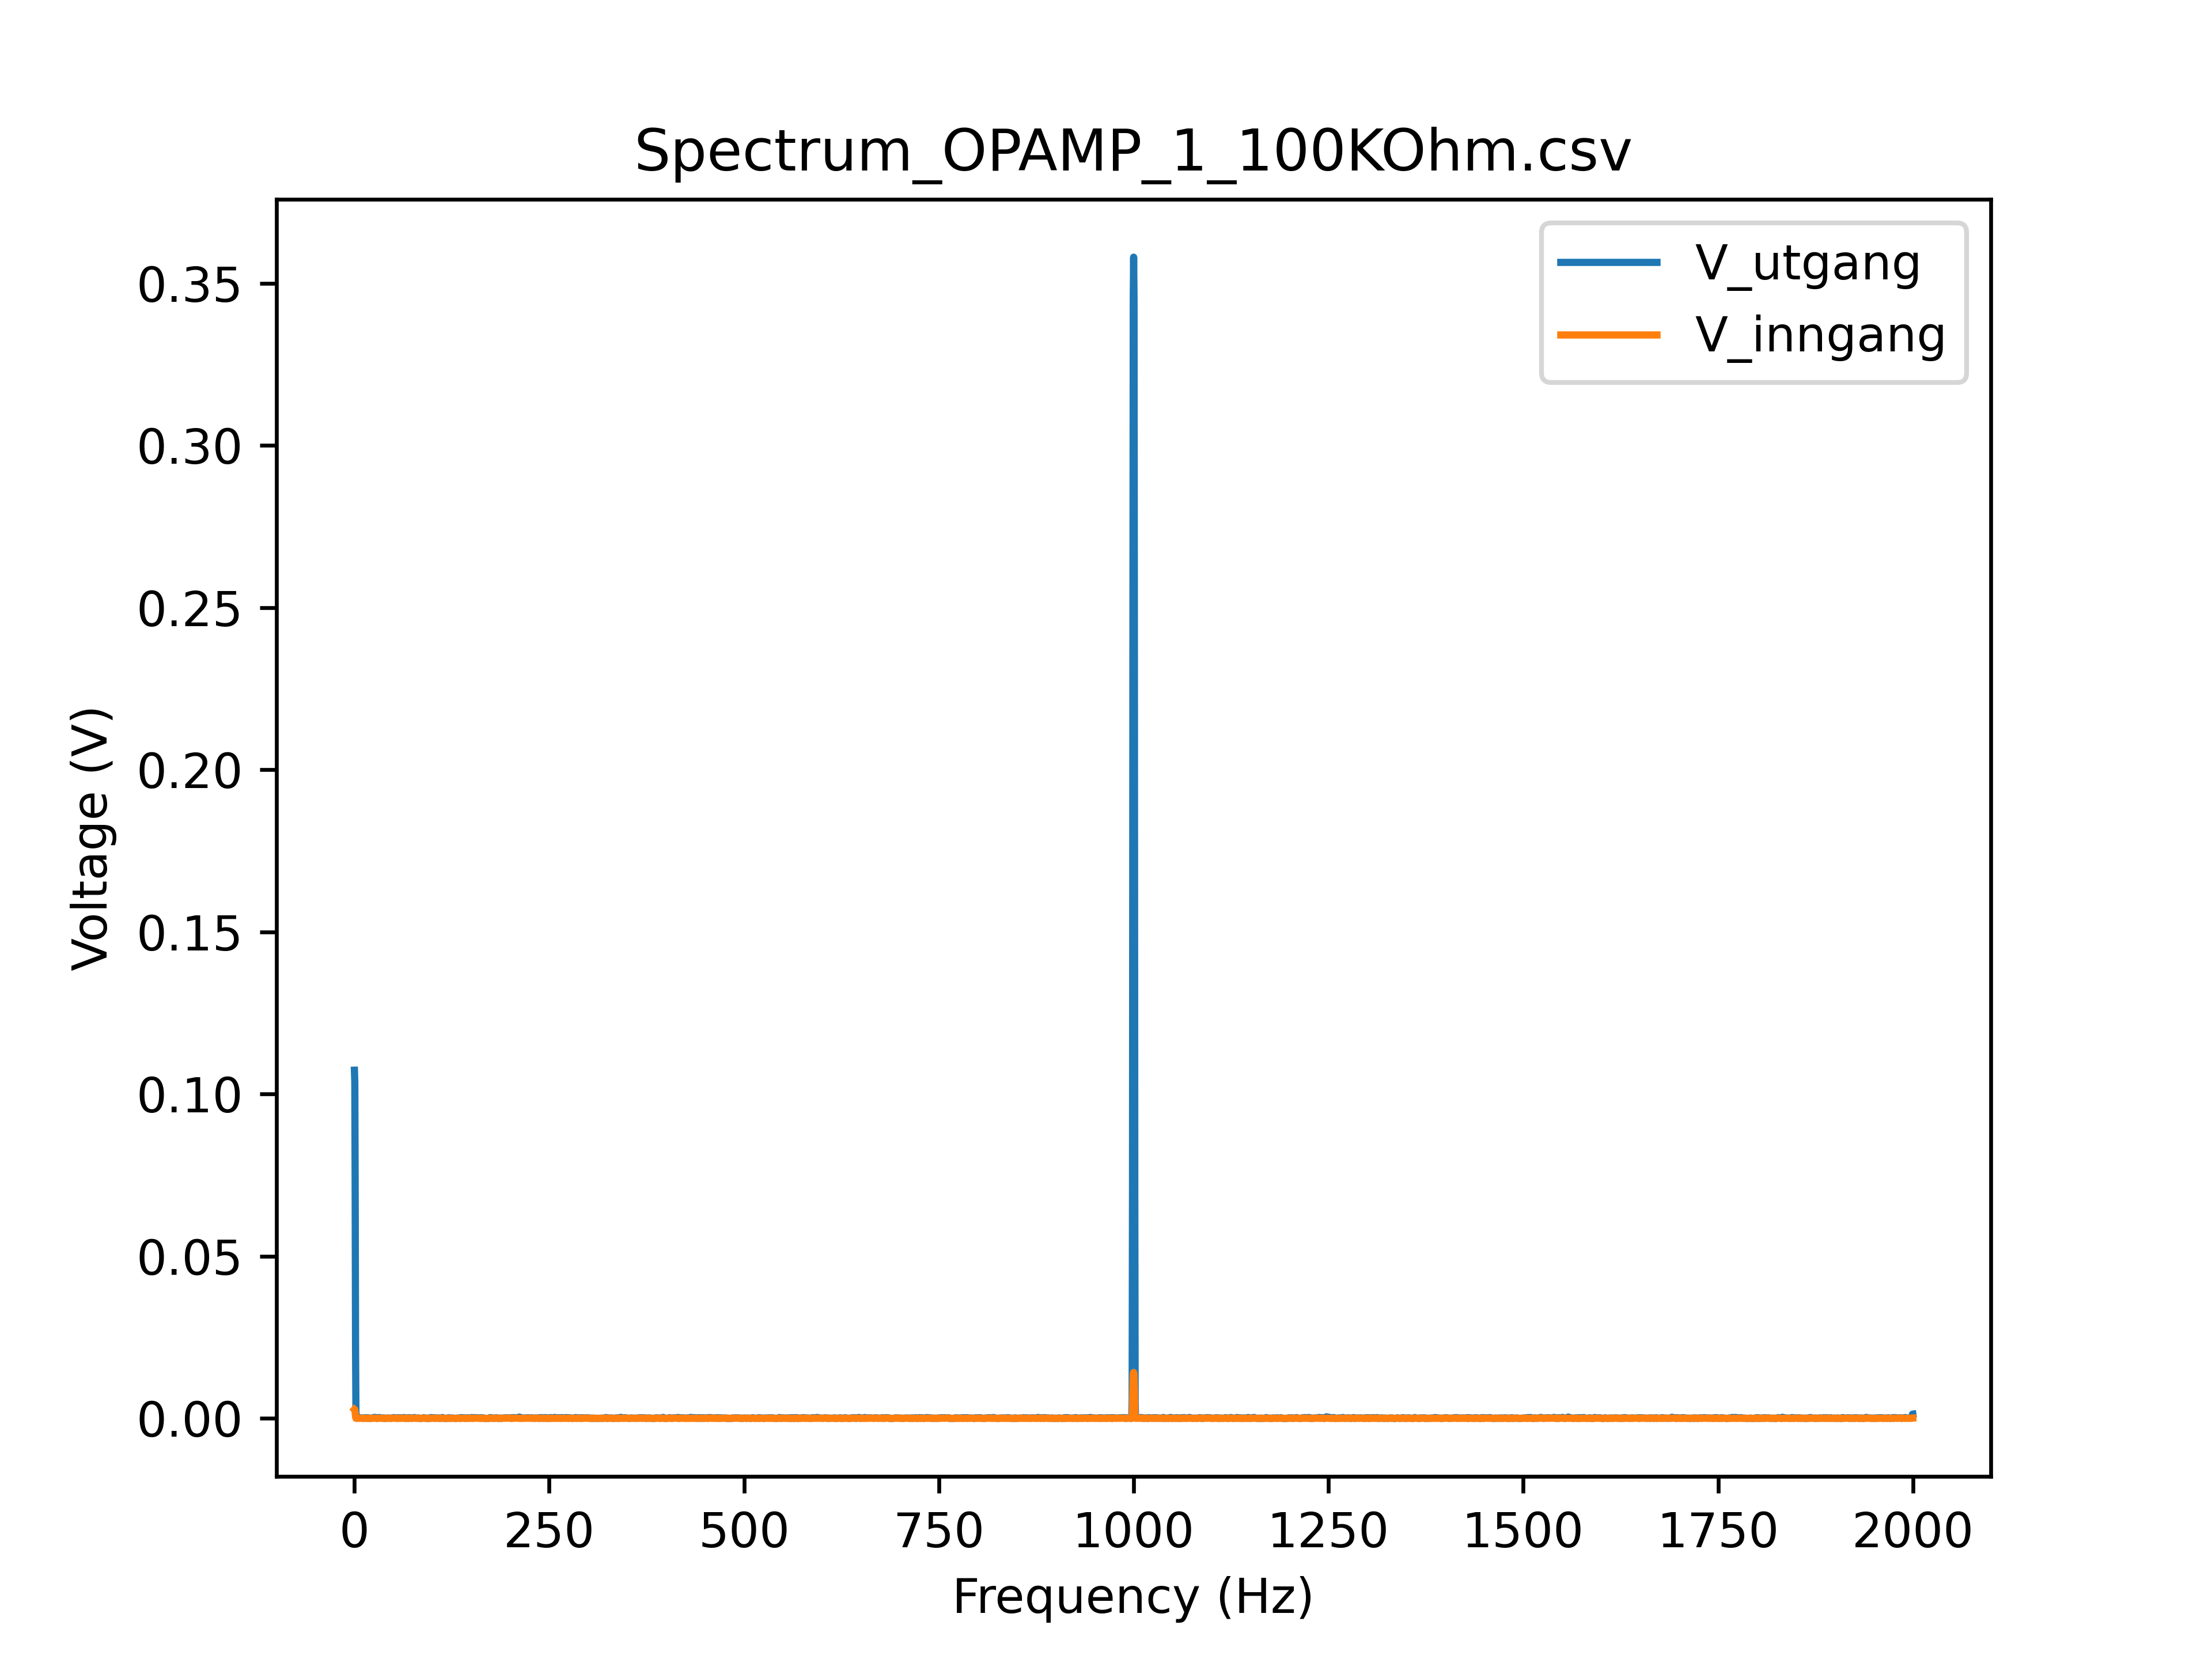
\includegraphics[width=1\textwidth]{Bilder/Spectrum_OPAMP_1_100KOhm.png}
        \caption{Spectrum med $R_L = 100k\Omega$\\ åpen løkke}
        \label{fig:Spectrum_OPAMP_1_100KOhm}
    \end{minipage}
    \hfill
    \begin{minipage}[c]{0.5\textwidth}
        \centering
        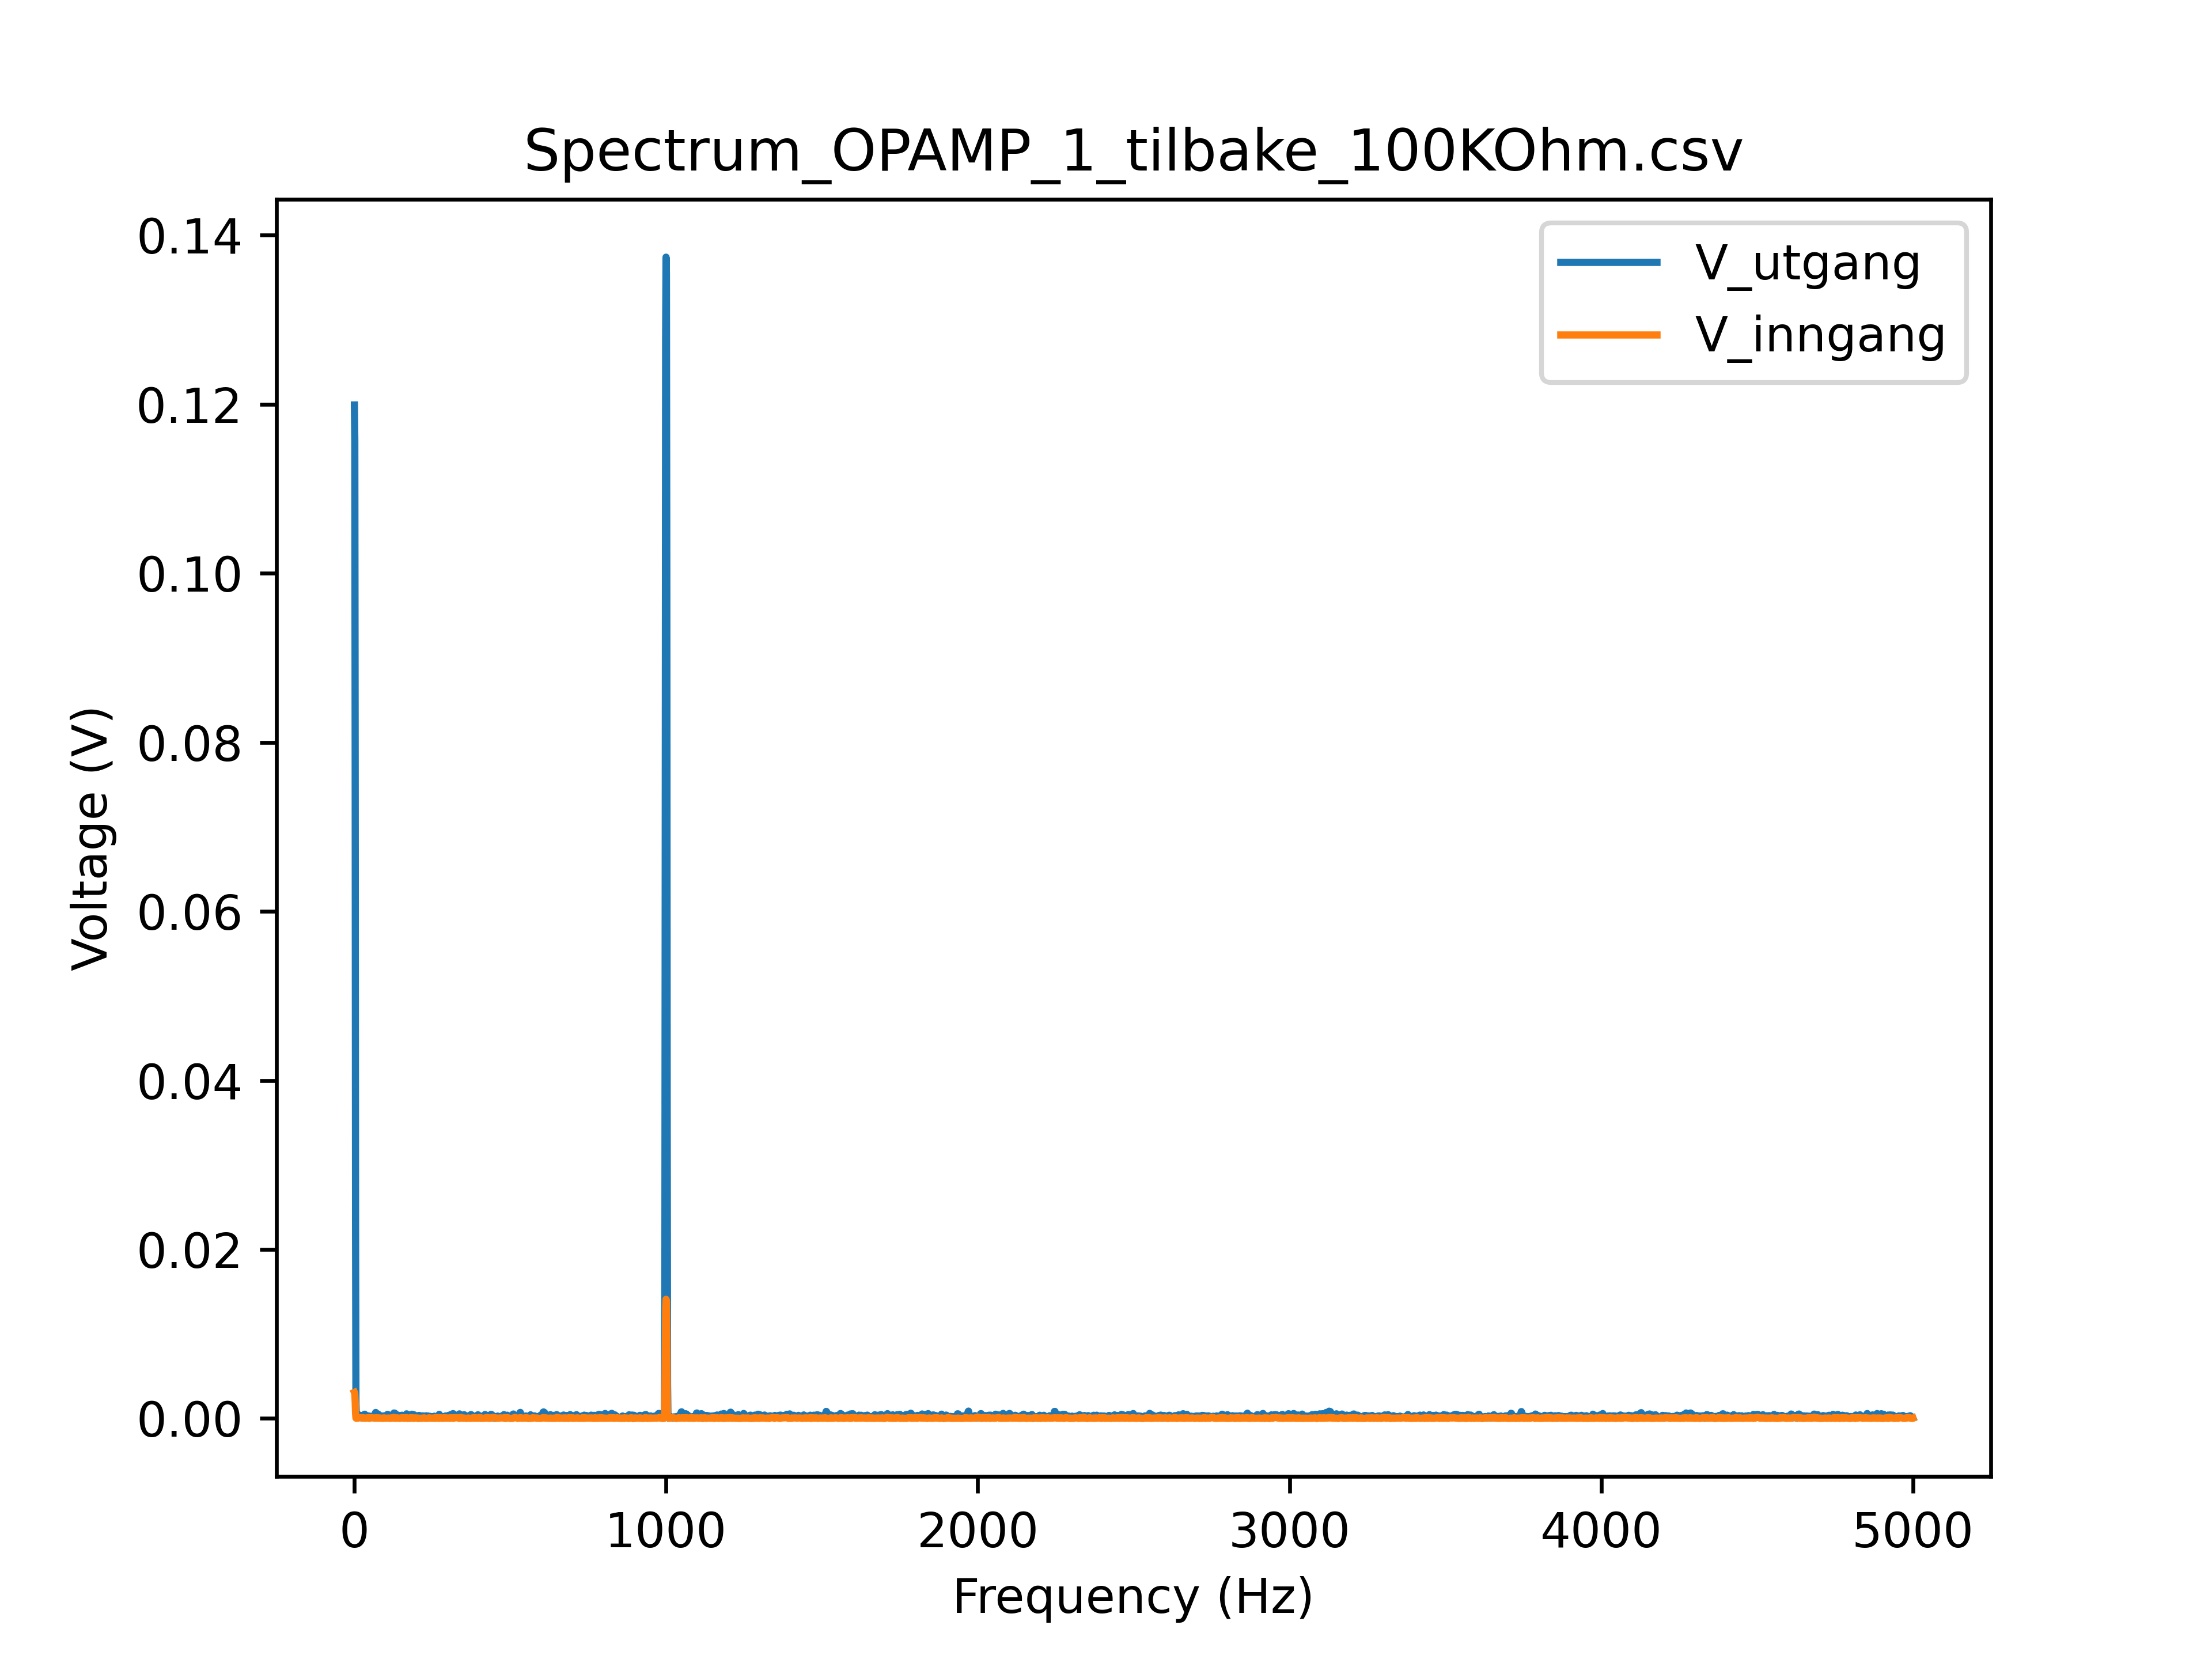
\includegraphics[width=1\textwidth]{Bilder/Spectrum_OPAMP_1_tilbake_100KOhm.png}
        \caption{Spectrum med $R_L = 100k\Omega$\\ tilbakekobling}
        \label{fig:Spectrum_OPAMP_1_tilbake_100KOhm}
    \end{minipage}
\end{figure}

Som vi ser i figur \autoref{fig:Spectrum_OPAMP_1_tilbake_100KOhm} så er det mye distorsjon ved 0Hz. Dette er fordi vi har en DC offset på utgangen. Dette kan vi fjerne ved å sette inn en kondensator i tilbakekoblingen. 

\subsection{Diskusjon av måleresultater}
\label{diskusjon}
Det som står mest ut blant målingene er de store frekvenskoponentene rett ved 0Hz i spektrumsanalysen. Dette er fordi vi har en DC offset på utgangen som forskyver signalene i forhold til hverandre noe som man enkelt kan se ved å se på ocilloskopsdataen som vist i \autoref{fig:ocilloskop_data} og \autoref{fig:ocilloskop_data_tilbake}. Ettersom dette har en veldig stor påvirkning på THD uten å egentlig bidra med noe støy så kan vi beregne THD uten å ta hensyn til DC offseten som vist i \autoref{tab:THD_and_Amplitude_Data}. Dette gjør vi ved å bruke \autoref{eq:THD} på dataen fra spektrumsanalysen ved hjelp av python koden under. Hadde man tatt med signalene på 0Hz så hadde THD blitt i snitt 200\% i motsetning til det som er vist i \autoref{tab:THD_and_Amplitude_Data}. 

\begin{figure}
    \begin{minipage}[c]{0.5\textwidth}
        \centering
        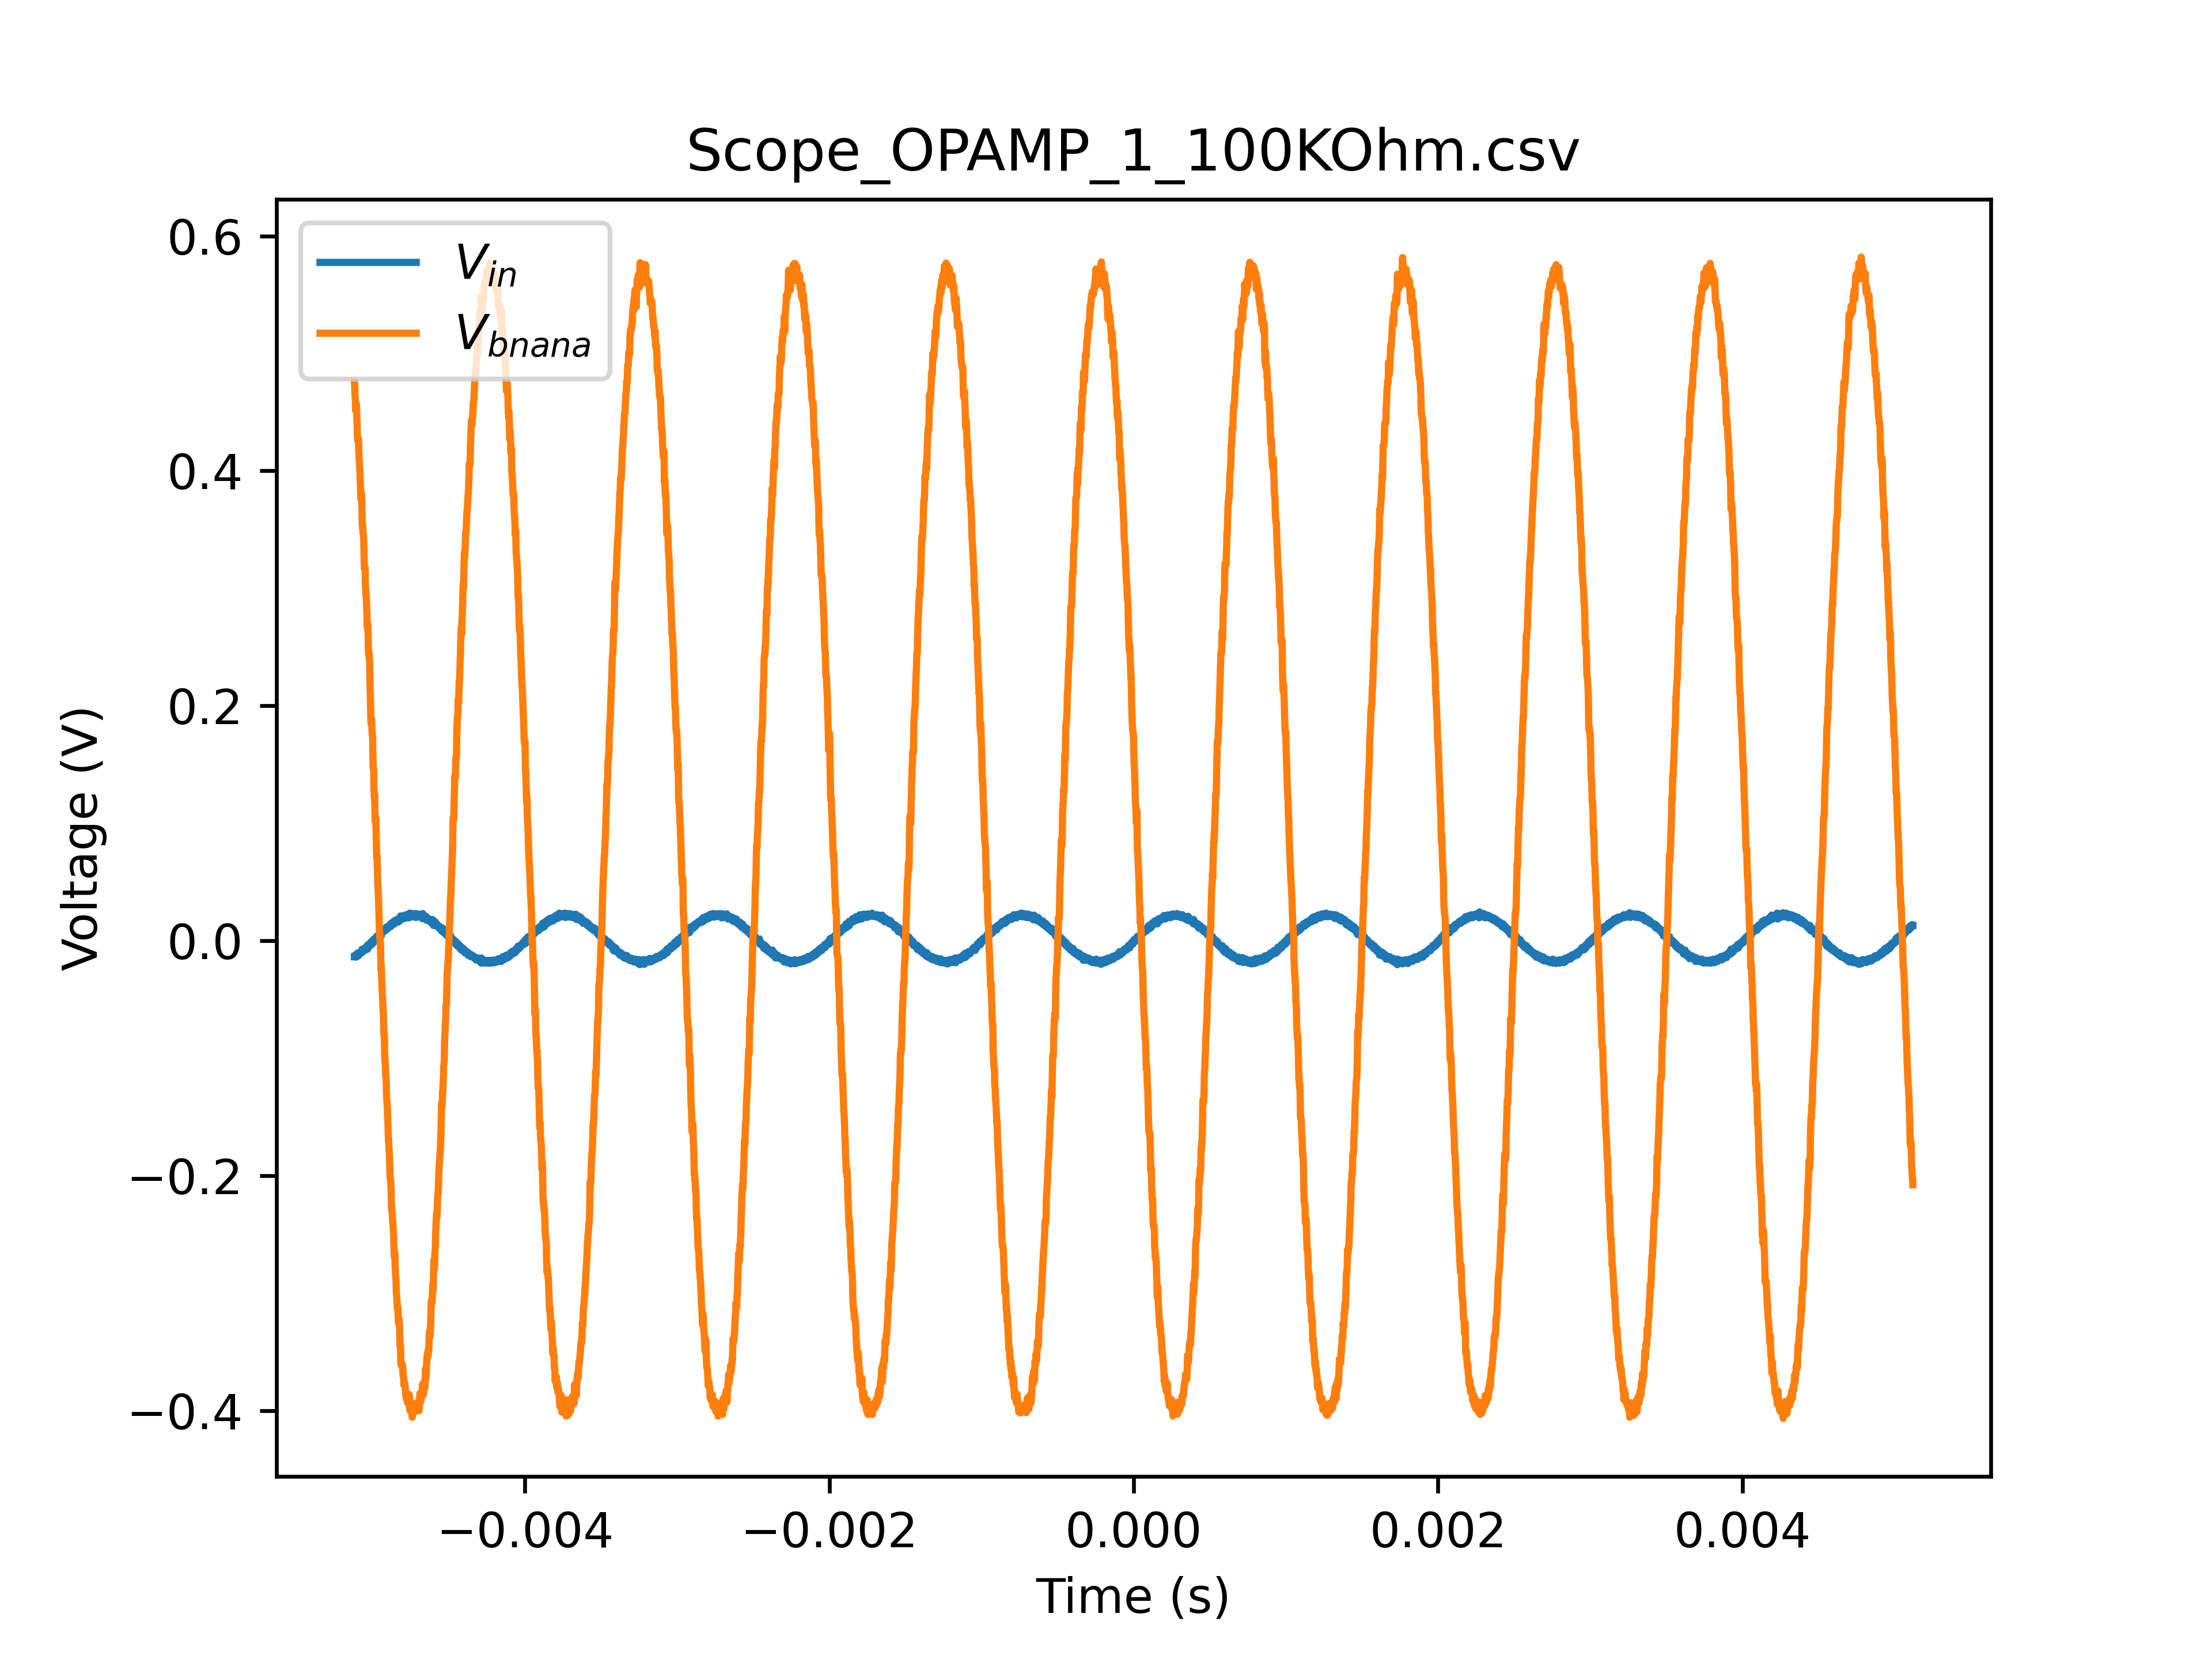
\includegraphics[width=1\textwidth]{Bilder/Scope_OPAMP_1_100KOhm.png}
        \caption{Ocilloskopsdata}
        \label{fig:ocilloskop_data}
    \end{minipage}
    \begin{minipage}[c]{0.5\textwidth}
        \centering
        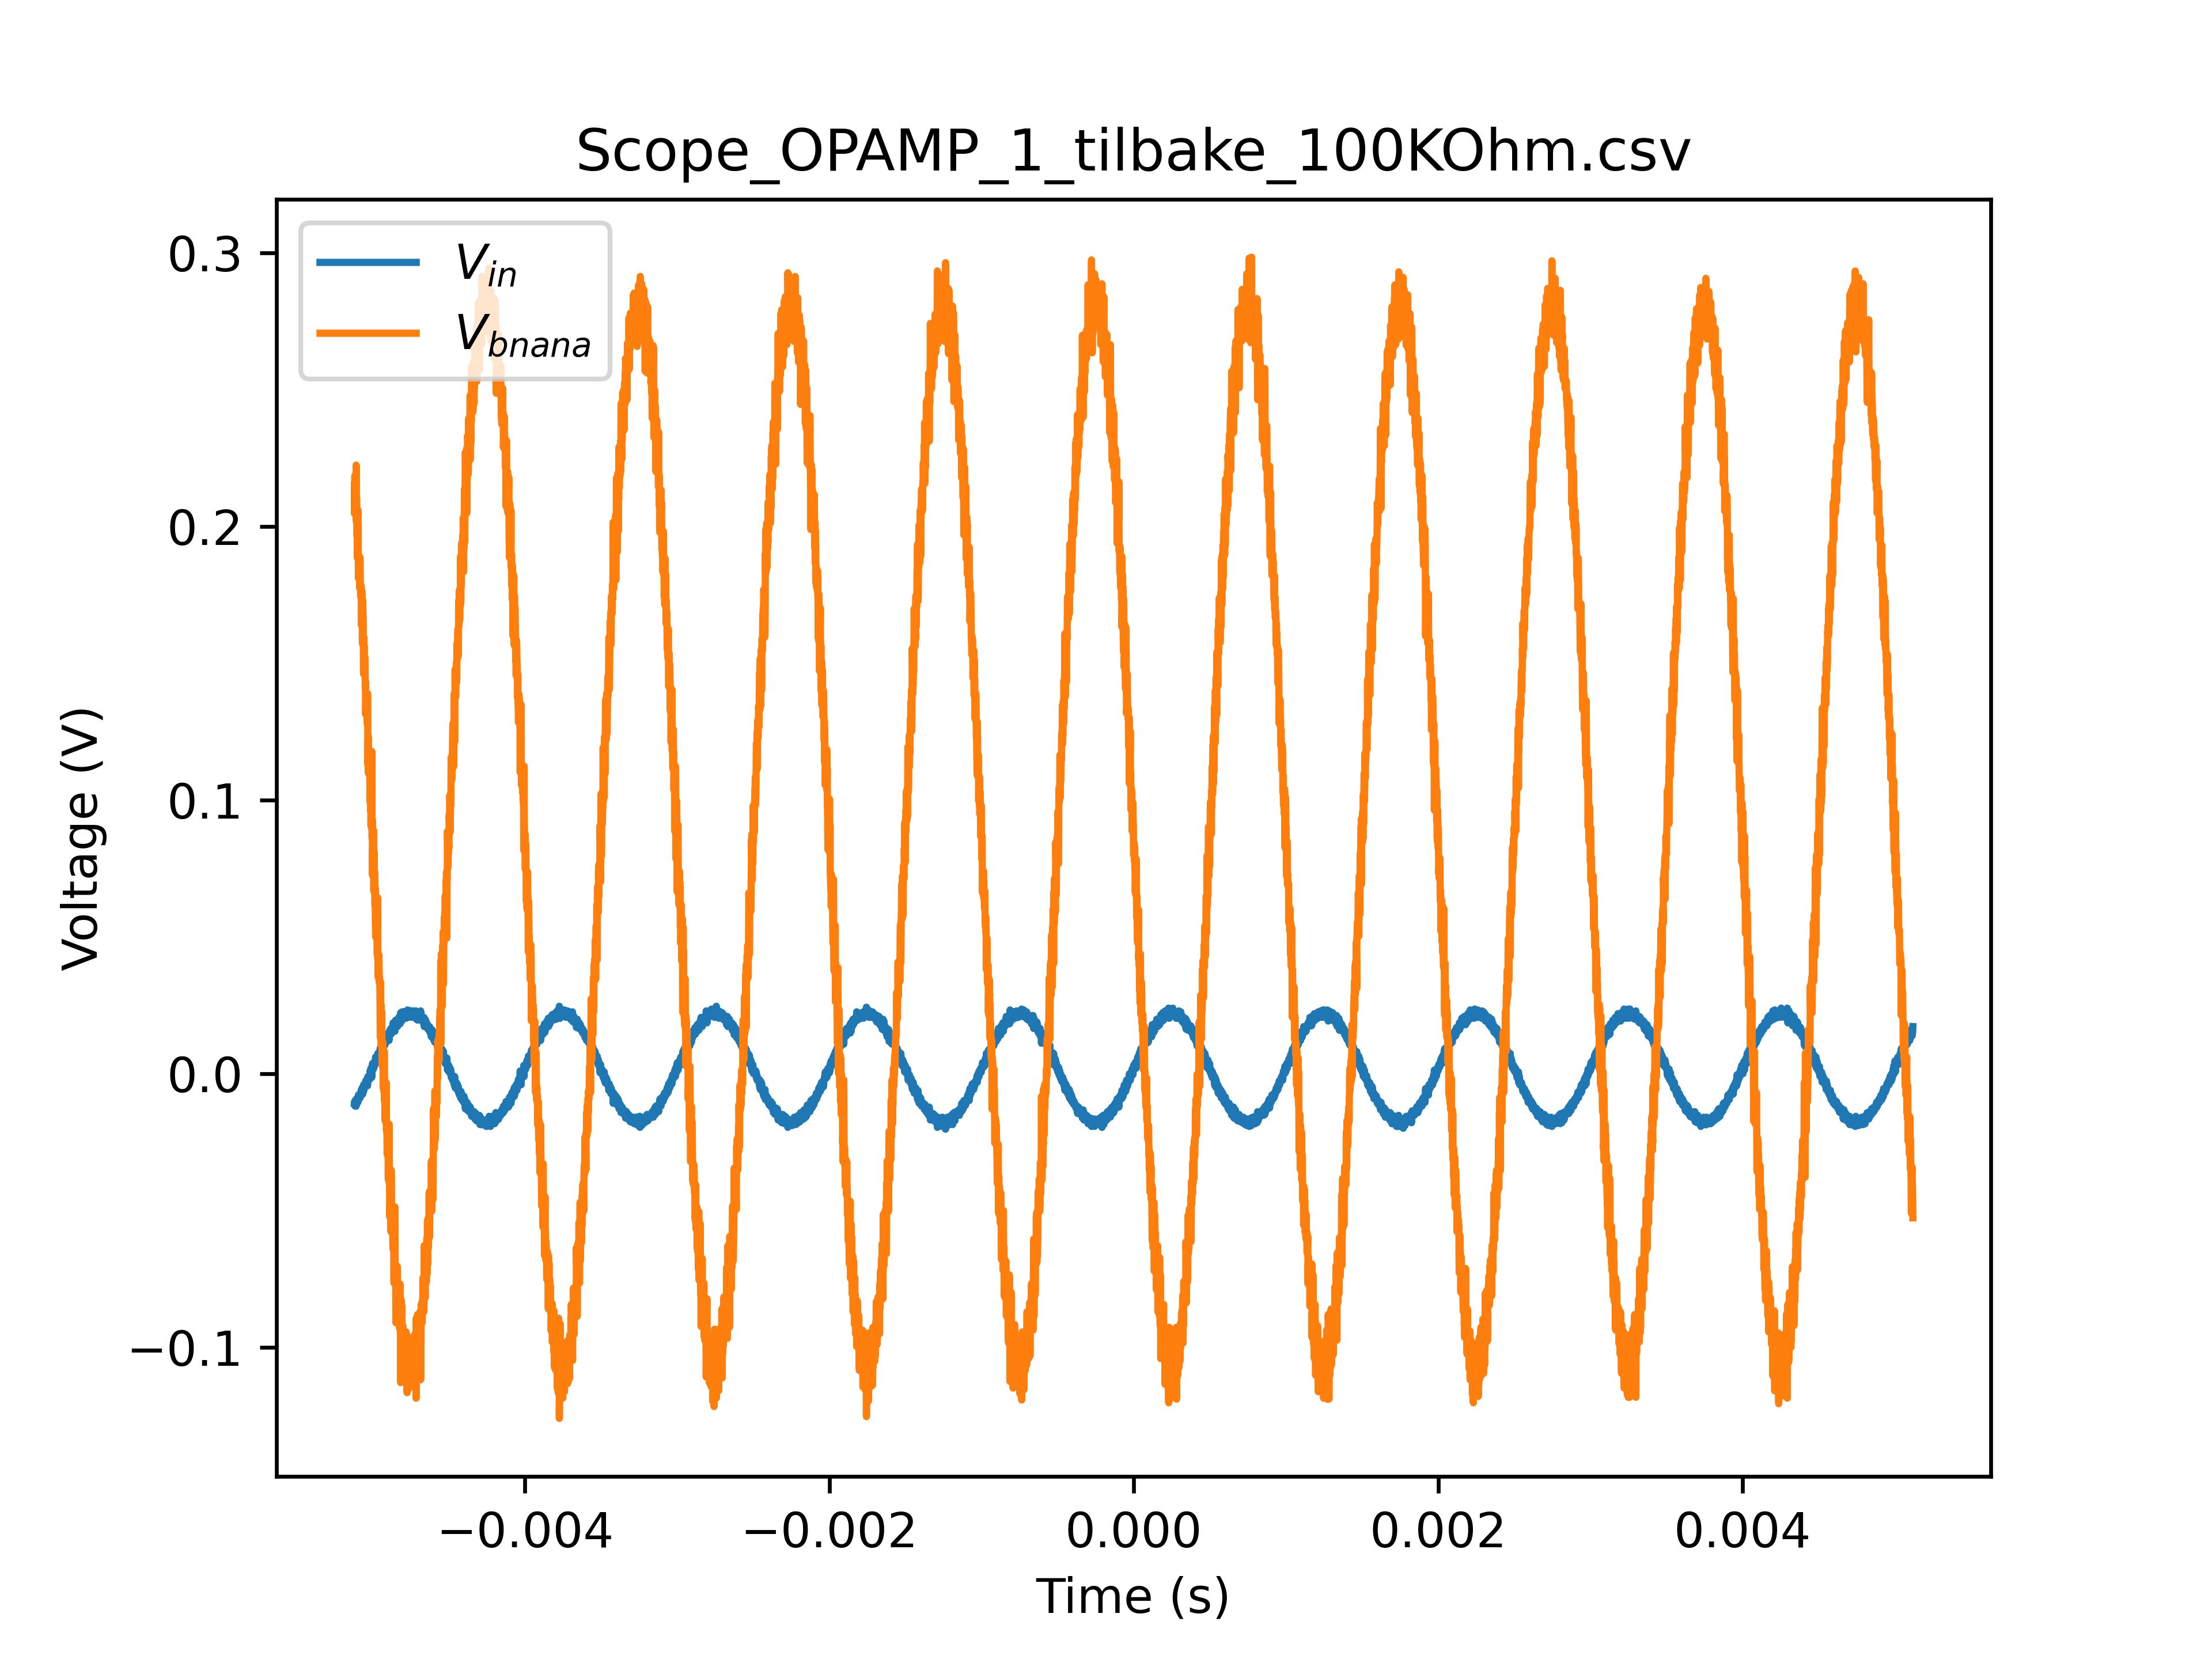
\includegraphics[width=1\textwidth]{Bilder/Scope_OPAMP_1_tilbake_100KOhm.png}
        \caption{Ocilloskopsdata med tilbakekobling}
        \label{fig:ocilloskop_data_tilbake}
    \end{minipage}
\end{figure}


\subsection{Forbedringer}
\label{forbedringer}
Denne kretsen kunne blitt bedre hadde man koblet opp en emitter følger ved utgangen, silk at kretsen hadde blitt seende ut som i \autoref{fig:forbedret_diffamp}. Denne endringen ville også sansyneligvis redusert THD ved å fjerne DC offseten på utgangen i tilleg til å sentrere utgangssignalet rundt 0V.

\begin{figure}[H]
    \centering
    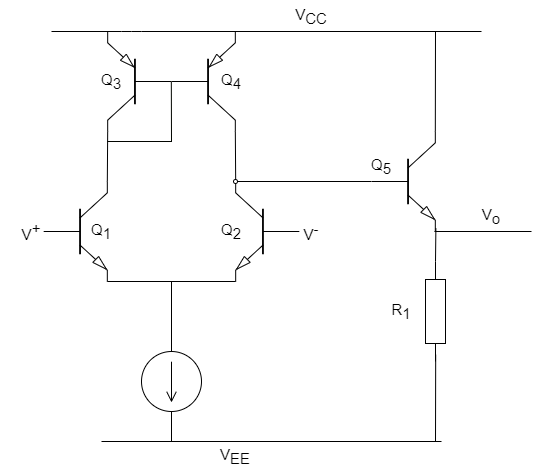
\includegraphics[width=0.7\textwidth]{Bilder/diffamp_V2.drawio.png}
    \caption{Forbedret differensialforsterker}
    \label{fig:forbedret_diffamp}	
\end{figure}
